%!TEX root = ../main.tex
\catalin{IMPORTANT: In case we get the actual network running, don't forget to change the text accordingly (implementation not successful etc.)}
\subsection{Methods to implement CAN on Linux}

The next step after testing the stack board and showing the basic functionality of the CAN network was to implement it using Linux running on the Zybo board.
This step required enabling the CAN drivers that reside in the Xillinux kernel and gaining access to the CAN devices.
This section describes the necessary procedures that were followed in order to gain control over the CAN network from Linux.
\\
At this point the reader should be informed that although the CAN controllers could be used on the Processing System using bare-metal code, the implementation of CAN on the Programmable Logic and the access to it from Linux was not successful.
After a lot of effort to create a physically functional network and researching on how to implement it, the conclusion that the available documentation is lacking was reached.
Alternatively, other means to prove the concept of the project were taken into account, as described in section \ref{sub:Utilizing_Svr_Virtualization}.

\subsubsection{Enabling the CAN Drivers}

This was the first idea on how to utilize the CAN network using Linux.
In order to enable the drivers on the Zynq7 Processing System, the Linux CAN driver guide \cite{Xilinx_wiki_Linux_CAN_driver} on the Xilinx wiki website \cite{Xilinx_wiki} was followed.
The Kconfig file under the path \ref{code:can_kconfig_pathfile} needed to be configured.
The entry at line 128 was changed as seen in the code snippet \ref{code:can_kconfig_contents_line128}.
Originally, lines 130 and 131 were as seen in the snippet \ref{code:can_kconfig_original_line130}.

\begin{lstlisting}[caption={CAN Kconfig pathfile.},numbers=none,label=code:can_kconfig_pathfile]
/usr/src/kernels/3.12.0-xillinux-1.3/drivers/net/can
\end{lstlisting}

\catalin{Xilinx CAN has "" around it, but LaTeX shows errors if inserted in the code snippet.}
\martin{Careful about the line length in the code}
\begin{lstlisting}[firstnumber=128,caption={Kconfig file contents from line 128.},label=code:can_kconfig_contents128]
config CAN_XILINXCAN
	tristate Xilinx CAN
	depends on NET [=y] && CAN_DEV [=y] && CAN [=y] && (ARCH_ZYNQ || MICROBLAZE [=y])
	default y
	---help---
	  Xilinx CAN driver. This driver supports both soft AXI CAN IP and
	  Zynq CANPS IP.
\end{lstlisting}

\begin{lstlisting}[firstnumber=130,caption={Original content of lines 130 and 131.},label=code:can_kconfig_original_line130]
	depends on CAN && (ARCH_ZYNQ || MICROBLAZE)
	default n
\end{lstlisting}

The next step of the process was the modification of the device tree settings file, requiring an entry for the CAN PS to be inserted.
The necessary file was located under the boot folder named as seen in \ref{code:dts_file_zybo}.
The modifications can be seen in the snippet \ref{code:dts_changes_zybo} for can controllers as well as for the AXI CAN core.

\begin{lstlisting}[numbers=none,caption={Device tree settings file and its path.},label=code:dts_file_zybo]
/boot/xillinux-1.3-zybo.dts
\end{lstlisting}
\catalin{Double quotes are problem here as well. FIX THEM WHENEVER}
\begin{lstlisting}[caption={Device tree settings changes.},label=code:dts_changes_zybo]
zynq_can_0: can@e0008000 {
        compatible = xlnx,zynq-can-1.0;
        clocks = <&clkc 19>, <&clkc 36>;
        clock-names = can_clk, pclk;
        reg = <0xe0008000 0x1000>;
        interrupts = <0 28 4>;
        interrupt-parent = <&intc>;
        tx-fifo-depth = <0x40>;
        rx-fifo-depth = <0x40>;
    };
axi_can_0: axi-can@40000000 {
        compatible = xlnx,axi-can-1.00.a;
        clocks = <&clkc 0>, <&clkc 1>;
        clock-names = can_clk,s_axi_aclk;
        reg = <0x40000000 0x10000>;
        interrupt-parent = <&intc>;
        interrupts = <0 59 1>;
        tx-fifo-depth = <0x40>;
        rx-fifo-depth = <0x40>;
        };
\end{lstlisting}

\mikkel{Maybe you can provide some thoughts about the problem. Maybe also some words about the patching Xilinx-Digilent etc.}
As was previously mentioned, the implementation was unsuccessful. At the time, the research done on this topic did not lead to successfully enabling the drivers.

\subsubsection{Utilizing the AXI CAN core}

Another way to implement a CAN network was to use the AXI CAN core that is available in the Vivado Suite, instead of gaining direct access to the CAN drivers.
Unfortunately due to a license restriction from Xilinx, the core can only be used for simulation purposes and not actual hardware implementations.
This information became available after the process of creating the bistream file in the form of an error, thus not allowing for further use of the core.
The architecture can be seen in figure \ref{fig:CAN_Arch_with_AXI_CAN}.
The core accepts a clock frequency from \SI{8}{\mega\hertz} to \SI{24}{\mega\hertz}, which in the block diagram is provided by the FCLK\_CLK1.

\begin{figure}[h!]
	\centering
	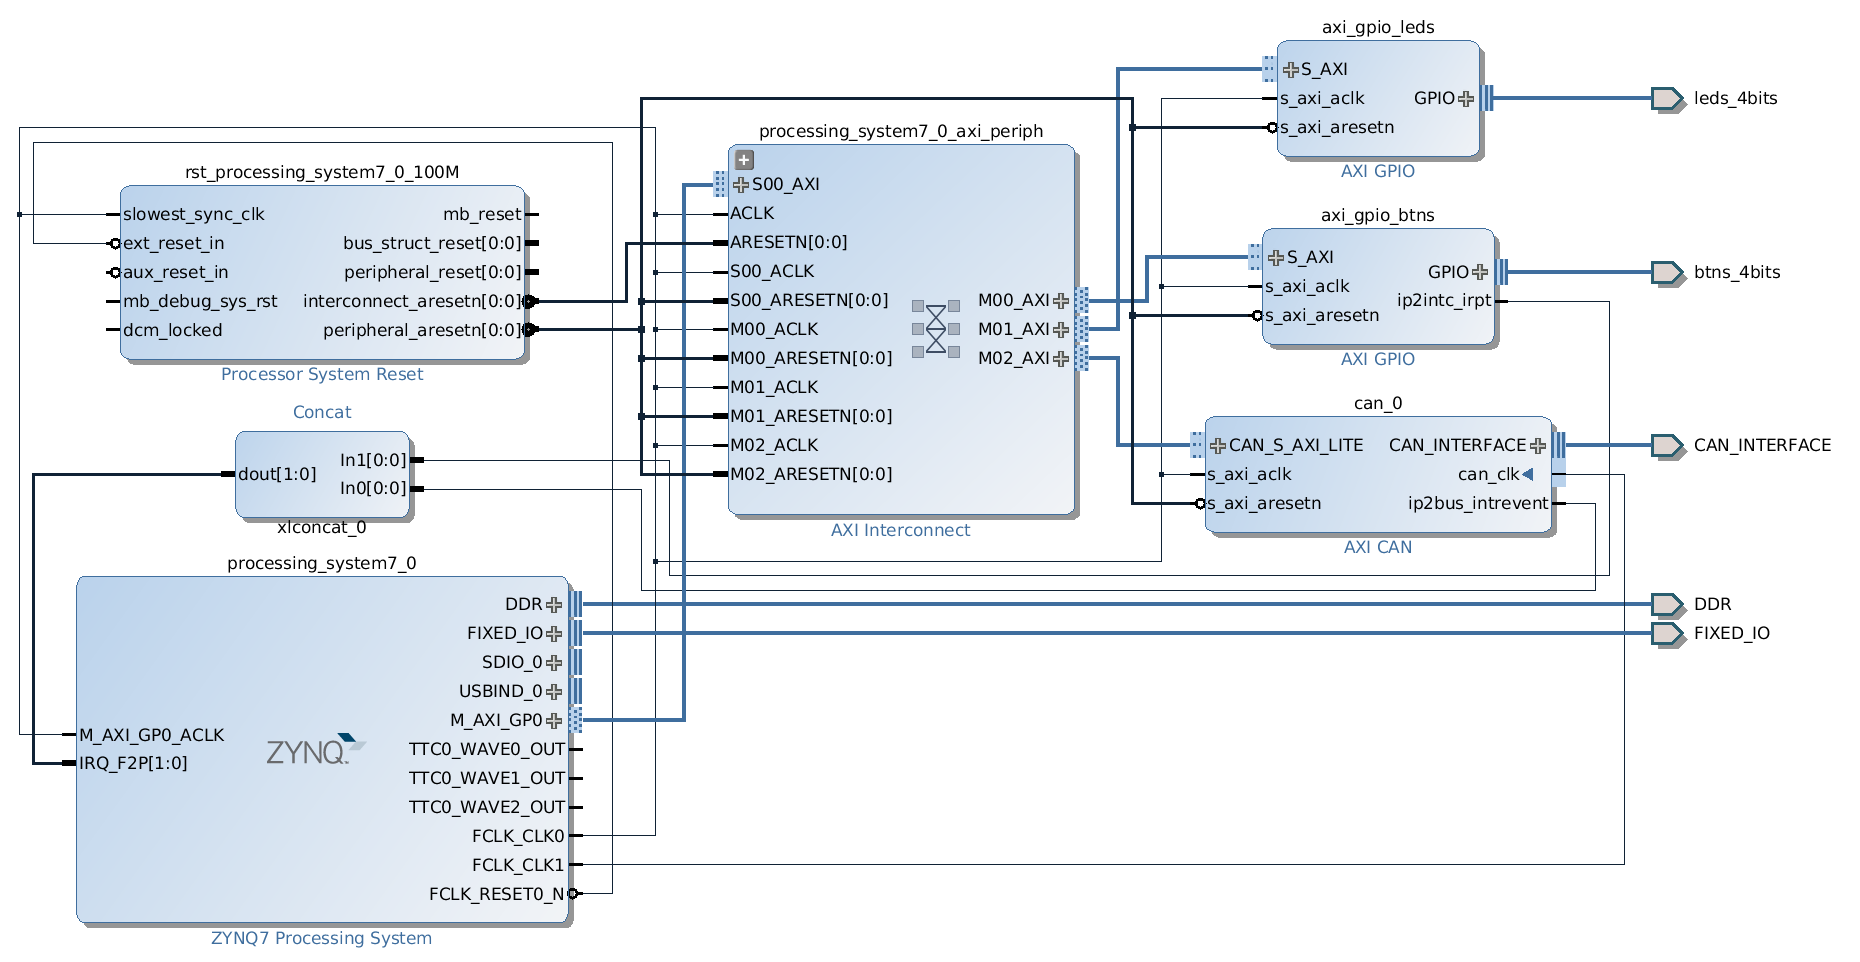
\includegraphics[width = 1.2\linewidth]{graphics/Zybo_Arch_with_AXI_CAN.png}
	\caption{Block diagram featuring the architecture in Vivado with the AXI CAN core.}
	\label{fig:CAN_Arch_with_AXI_CAN}
\end{figure}

\subsubsection{Utilizing Asymmetric Multiprocessing}

Apart from using the AXI CAN core and the CAN drivers, the Zynq-7000 AP SoC provides the possibility of implementing a mechanism called asymmetric multiprocessing since there are two processors which share common memory as well as peripherals.
The idea of this is to run Linux OS on one processor, while on the other one a bare-metal system, which both of them can communicate with each other.
This was a proposed solution for the problem of accessing the CAN devices from Linux which was the most promising of the implementation methods discussed in this report, but due to lack of time, it was researched only at a theoretical level.
A brief implementation description will be give in this section, but for more details about the instructions and applications, the reader may refer to the Xilinx document \cite{Xilinx_AMP}.

\paragraph{Implementation details}~\\
In order to achieve asymmetric multiprocessing on the Zybo board, certain steps are required to be taken, but also a few precautions as well.
An important one is to configure the two processors appropriately in order to use the shared memory without conflicts.
A second one is to setup the CPU0 as the master, because that is the processor assigned for the Linux OS.
It is also the one that will start CPU1 by writing a value to a specific address in memory.
Also, Linux needs to be configured as symmetric multiprocessing with a maximum number of one CPUs.
It is a good approach because it will ensure that Linux configures the interrupt control distributor (ICD) and the snoop control unit (SCU) appropriately for multi-CPU environment, but only running on one of the two CPUs.
\\
Applications for the bare-metal and the Linux part are also needed. Specifically, the former makes use of the fist stage boot loader (FSBL) as well as a custom application that will run on the CPU1 after it will be loaded by the FSBL into the memory.
The latter, the Linux OS, uses two applications as well.
The first one is RWMEM which is an utility providing the ability to read and write to various memory locations.
The second one is the Soft UART, which constantly monitors the memory in order to receive data from the application running on the second processor, the bare-metal code.
\\
The next step is to create the Linux kernel and device tree, as well as the u-boot.
Acquiring the root file system is also a requirement.
One important note here is the modification of the device tree includes instructions for the Linux to only use one CPU and to not access certain amount of memory, which is reserved for the bare-metal application.
For instructions for the creation of the kernel, u-boot and acquiring the root file system, the reader may refer to the Xilinx Wiki \cite{Xilinx_wiki}.
\\
Lastly, after all the above steps, the last one is to follow the appropriate procedures to copy the necessary files to an SD card. The files, including the applications, are:
\begin{itemize}
\item BOOT.BIN
\item uramdisk.image.gz
\item devicetree.dtb
\item uImage
\item rwmem.elf
\item softUart.elf
\end{itemize}

The application for the CPU1 is included in the BOOT.BIN file.

\subsubsection{Using can-utils for virtual nodes}

During the development of this project, the can-utils tool was also used.
It is a testing tool that can be executed on Linux and can be applied on real as well as virtual CAN devices.
Initially it was used to create a virtual network with two nodes locally on a computer to gain a better understanding of how CAN networks function and how they can be configured.
It was also intended to be used to test the actual network, but since the network was not implemented, further use of the tool was not necessary.
\catalin{Rerun some virtual tests with can-utils to get code snippets}

\subsubsection{Utilizing Service Virtualization for the Proof of Concept}
\label{sub:Utilizing_Svr_Virtualization}

In order to show that the system can be fully functional despite the unsuccessful attempt to implement it, a different approach than the actual implementation is needed.
One way of doing that is to apply a method called service virtualization where one part of the system can be simulated to prove that the rest of the system is fully functional, given the presence of the missing simulated part.
\\
In this case, the system that was designed for this project can be divided into two parts or subsystems.
The first one is the physical CAN network that was proved functional using bare\-metal code programmed using the JTAG mode \catalin{is this well expressed, JTAG mode?} on the Zybo board in the section \ref{sub:TestingCANStack_BareMetal}.
The second part would be considered the subsystem present on Linux which included the protocol designed to be used with the CAN bus and the application which extracted the data from the sensors.
\catalin{Some more words about how are we going to produce the data and how are we going to pass the data to the application etc.}
The main idea was to run three tests separately, which combined together would prove that the system is fully functional given the fact that there would be access to the CAN controller and physical network from Linux. In other words, a virtualized connection or link between the Linux OS running on the Zybo board and the CAN devices on the Programmable Logic level \catalin{can controllers or devices or sth else?} was simulated.
\catalin{more to add and modify when Thomas makes an awesome illustration for this.}
\catalin{How many tests in total for this proof of concept?}
